\documentclass[tikz]{standalone}
\usetikzlibrary{calc,arrows}
\usepackage{frenchmath}

\begin{document}
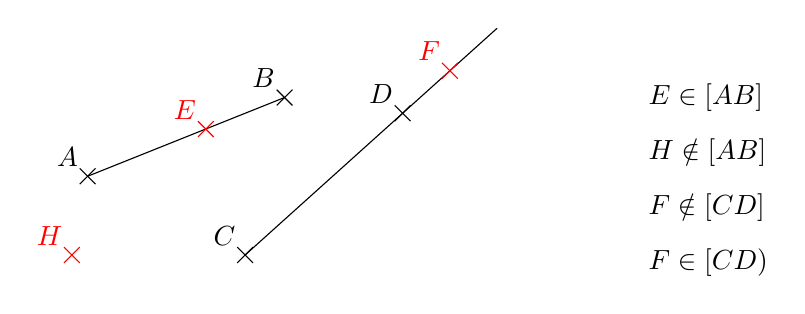
\begin{tikzpicture}
    \coordinate (A) at (0,0);
    \coordinate (B) at (2.5,1);
    \coordinate (C) at (2,-1);
    \coordinate (D) at (4,0.8);
    \coordinate (E) at ($(A)!0.6!(B)$);
    \coordinate (F) at ($(C)!1.3!(D)$);
    \coordinate (H) at (-0.2,-1);
    \draw[black] (A) -- (B);
    \draw[black] (C) -- ($(C)!1.6!(D)$);
    \draw ($(A)+(-0.1,-0.1)$) -- ($(A)+(0.1,0.1)$);
    \draw ($(A)+(0.1,-0.1)$) -- ($(A)+(-0.1,0.1)$);
    \draw ($(B)+(-0.1,-0.1)$) -- ($(B)+(0.1,0.1)$);
    \draw ($(B)+(0.1,-0.1)$) -- ($(B)+(-0.1,0.1)$);
    \draw ($(C)+(-0.1,-0.1)$) -- ($(C)+(0.1,0.1)$);
    \draw ($(C)+(0.1,-0.1)$) -- ($(C)+(-0.1,0.1)$);
    \draw ($(D)+(-0.1,-0.1)$) -- ($(D)+(0.1,0.1)$);
    \draw ($(D)+(0.1,-0.1)$) -- ($(D)+(-0.1,0.1)$);
    \node[above left] at (A) {$A$};
    \node[above left] at (B) {$B$};
    \node[above left] at (C) {$C$};
    \node[above left] at (D) {$D$};
    \draw[red] ($(E)+(-0.1,-0.1)$) -- ($(E)+(0.1,0.1)$);
    \draw[red] ($(E)+(0.1,-0.1)$) -- ($(E)+(-0.1,0.1)$);
    \draw[red] ($(F)+(-0.1,-0.1)$) -- ($(F)+(0.1,0.1)$);
    \draw[red] ($(F)+(0.1,-0.1)$) -- ($(F)+(-0.1,0.1)$);
    \draw[red] ($(H)+(-0.1,-0.1)$) -- ($(H)+(0.1,0.1)$);
    \draw[red] ($(H)+(0.1,-0.1)$) -- ($(H)+(-0.1,0.1)$);
    \node[above left,red] at (E) {$E$};
    \node[above left,red] at (F) {$F$};
    \node[above left,red] at (H) {$H$};
    \node[anchor=west] at (7,1) {$E \in [AB]$};
    \node[anchor=west] at (7,0.3) {$H \notin [AB]$};
    \node[anchor=west] at (7,-0.4) {$F \notin [CD]$};
    \node[anchor=west] at (7,-1.1) {$F \in [CD)$};
\end{tikzpicture}
\end{document}